\chapter{Solutions}
\renewenvironment{Figure}
  {\par\medskip\noindent\minipage{\linewidth}}
  {\endminipage\par\medskip}


\eocesolch{Introduction to data}
\begin{multicols}{2}

\eocesol{(a)~Ordinal (b)~Ordinal or Continuous  (c)~Nominal
  (d)~Continuous (e)~Discrete (f)~Nominal (g)~Nominal (h)~Discrete 
(i)~Nominal (j)~Nominal (k)~Continuous (l)~Continuous (m)~Continuous
(n)~Nominal (o)~Continuous (p)~Nominal (q)~Discrete (r)~Nominal
(s)~Nominal 
}
 
\eocesol{
 (a)~10--percentile=41.10 ; 35--percentile=44 ; 62--percentiles= 51.22 \setcounter{enumi}{2}
 (b)~$Q_1=$43.00; $Q_2=$48.00; $Q_3=$ 53.25 \setcounter{enumi}{1}
 (c)~$IQR=$10.25. Lower limit= 27.625; Upper limit=68.625. There is not outlying value. 
 (d)~Fig.\ref{fig:ex1.2}
  
}%%%\end{problem}
\begin{Figure}
      \begin{center}
    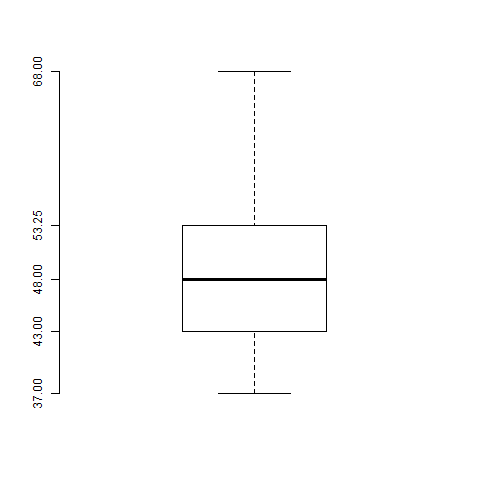
\includegraphics[width=0.9\textwidth]{extraTeX/appendix/TeX/ex3/boxplotEx2.png}
  \end{center}
    \captionof{figure}{ \label{fig:ex1.2} Boxplot Exercise 1.2 }
  \end{Figure}
\eocesol{
 (a)~Quantitative (discrete)
\newline
 (b)~ \begin{tabular}[t]{|*{7}{c|}}
\hline      0 & 1&  2 &  3  & 4  & 5  & 6 \\ 
\hline 7 &4 &6 &7 &4 & 4  & 8 \\
\hline 
    \end{tabular}
\newline
 (c)~The value 6. 
}%%%\end{problem}

\eocesol{
  
  (a)~The study variable is the moment of the day when emergency occurs. Qualitative nominal. 
 (b)~No, because it is a qualitative variable. \newline
 (c)~\begin{tabular}[t]{*{4}{c}}
 \hline   Afternoon   &  Morning  &    Night & Nonworking \\
  \hline       9       &  11  &         7  &         5 \\
\hline  0.2813   &  0.3438 &   0.2188 &   0.1563 \\
  \end{tabular}
\newline
 (d)~Fig.~\ref{fig:ex4}
  \begin{Figure}
  \begin{center}
    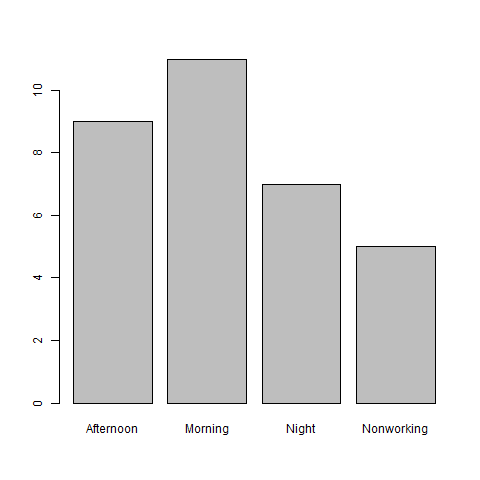
\includegraphics[width=0.9\textwidth]{extraTeX/appendix/TeX/ex3/barplotEx4.png}
  \end{center}  
\captionof{figure}{\label{fig:ex4} Bar plot exercise }
  \end{Figure}
}%%%}%%%\end{problem}
\eocesol{
  (a)  Copper levels in urine. Quantitative continuous
  (b) Median=0.71; Range=1.24-0.1=1.14
  (c) $Q_1=$0.5425; $Q_3=$0.8350  
  (d) 10-percentile=0.414  ; 95-percentile= 1.122
 (e) IQR=0.2925; Lower limit= 0.10375; Upper Limit= 1.27375; The value 0.1 is an outlying value 
 (f) Fig.~\ref{fig:ex5hist}  and \ref{fig:ex5box}  
}%%%\end{problem}

\begin{Figure}
 \begin{center}
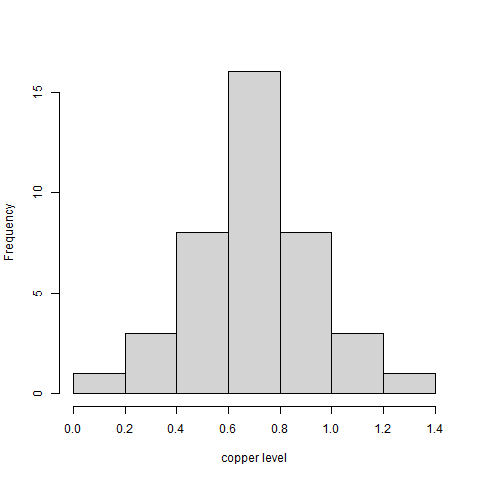
\includegraphics[width=0.9\textwidth]{extraTeX/appendix/TeX/ex3/histEx5.png} 
  \end{center}
  \captionof{figure}{\label{fig:ex5hist} Histogram Exercise 5}
\end{Figure}
\begin{Figure}
    \begin{center}
    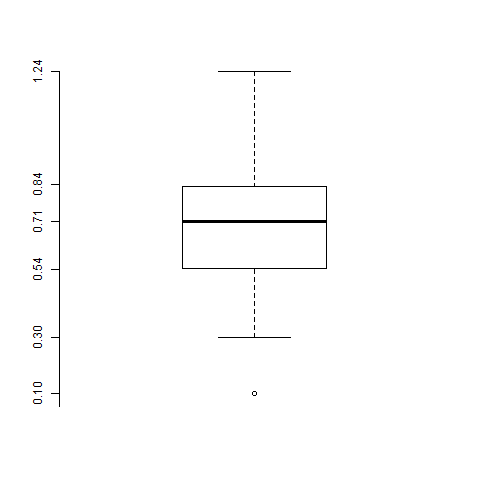
\includegraphics[width=0.9\textwidth]{extraTeX/appendix/TeX/ex3/boxplotEx5.png}
  \end{center}
  \captionof{figure}{\label{fig:ex5box} Boxplot}
\end{Figure}
\eocesol{
(a)~Qualitative continuous 
(b)~minimum and maximum; 3281 and  4422\newline 
 10 and 90 percentiles:3682.5 and 4288.0 ; \newline
 quartiles, median: $Q_1=$ 3955.75; $Q_2=$4125.00 $Q_3=$ 4173.00 \newline 
mean=4033.438\newline
mode ( It is not appropriate for a qualitative continuous variable) \newline range= 1141 \newline 
variance=82981.2, \newline 
standard deviation=288.0646
}%%%\end{problem}

\eocesolch{Probability and Distributions of Random Variables}


\eocesol{
 0.34+0.54-0.25=0.63
}%%%\end{problem}
\eocesol{
  (568-28)/568=540/568=0.9507
}%%%\end{problem}
\eocesol{
 $P(B\cap D)=0.15\cdot 0.24=0.036$
and $$P(B\cup D)=P(B)+P(D)-P(B\cap B)=0.15+0.24-0.036=0.354 $$
}%%%\end{problem}
\eocesol{
  Yes, because $P(A\cap B)=P(A)\cdot P(B)$
}%%%\end{problem}
\eocesol{
i) 0.4332; ii) 0.3445; iii) 0.9875; iv) 0.4920; v) 0.3174; vi) 0.2728;
vii) 0.0456; viii) 0.5886
  }
\eocesol{
  i)0.35; ii)1.54; iii) 2.16 iv) -1.24
}%%%\end{problem}
\eocesol{
  i)0.9970; ii) 0.0668 ; iii) 0.0873
}%%%\end{problem}
\eocesol{
  31.92\%
}%%%\end{problem}
\eocesol{
  95.44\%
}%%%\end{problem}
\eocesol{
The 80-percentile is 73.4. So, the answer is 
  74
}%%%\end{problem}
\eocesol{
 The lenght 6 feet is equivalent to 72 inches. \newline 
 $P(X<72)=P(Z<4/3)=0.9082$
}%%%\end{problem}
\eocesol{
  i)1.70\%; ii) 85.55
}%%%\end{problem}
\eocesol{
 i)  (3.08,10.92); ii) (2.34,11.66); iii) $(3.72,+\infty)$;\newline 
 iv) 4\%; 
v) 89.44\%; vi) 38.30\%; \newline 
vii) 9.19\% viii) 96 percentile
}%%%\end{problem}

\eocesol{
  i) (126.48,173.52); ii) (130.32,169.68); iii) (0,169.68) \newline
  iv) 74.86\%; v) 77.34\%; vi) 74.92\% ; vii) 98.12 percentile
}%%%\end{problem}
\eocesolch{Chapter 3}




%_______________

%% 4.1 SAMPLING VARIABILITY

% 1 oi_biostat, blue_eggs

\eocesol{(a)~$\overline{x} = 0.6052.$ \\
	(b)~$s = 0.0131$. \\
	(c)~$Z_{0.63} = \frac{0.63 - 0.6052}{0.0131} = 1.893$. No, this level of BGC is within 2 SD of the mean. \\
	(d)~The standard error of the sample mean is given by $\frac{s}{\sqrt{n}} = \frac{0.0131}{\sqrt{70}} = 0.00157$.
}

% There is not section with exercises\par
 \eocesolch{Chapter 4}


\eocesol{
 $80.5\pm 14.2\cdot 1.96 /\sqrt{24}$. The 95- CI is   $(74.8188,86.1812)$ 
}%%%\end{problem}
\eocesol{
$85=110(1-\alpha)$; $\alpha=0.15$; $1-\alpha/2=0.925$ and
$z_{0.925}=1.44$.

The error $z_{1-\alpha/2} \sigma /\sqrt{n}$ is less than $2.75$. Hence
$$n> z_{1-\alpha/2}^2\frac{\sigma^2 }{2.75^2}=1.44^2\frac{86.4}{2.75^2}=23.69$$  
  The sample size should be larger that 24. 
}%%%\end{problem}

\eocesol{
  $90\pm 1.96\cdot10/\sqrt{49}$. The 95-CI is $(87.2,92.8)$ 
}%%%\end{problem}

\eocesol{
  $\bar{x}=80.1333$ and $s=5.4099$. $t_{14,.975}=2.145$. \newline
$80.13\pm 2.145\cdot 5.4099/\sqrt{15}$ The 95-CI is
$(77.1371,83.1285)$. 
}%%%\end{problem}

\eocesol{
  $n=100>30$; $\bar{x}=23$; $s=10$; $100(1-\alpha)=90$; $\alpha=0.1$;
  $1-\alpha/2=0.95$; $ z_{.95}=1.64$ \newline 
$23\pm 1.64{\color{red} \cdot} 10/\sqrt{100}$. The 90\%-CI is $(21.36,24.64)$   
}%%%\end{problem}

\eocesol{
  Assuming that the weight of ten year-old male gorilla is a normal
  variable.

 $\alpha=0.1$ and $t_{24,.95}=1.711$

$36.5\pm 1.711{\color{red} \cdot} 5/\sqrt{25}$. The 90-CI is $(34.789,38.211)$.
}%%%\end{problem}

\eocesol{  %PROBLEM 7
 % $\bar{x}=12$; $n=10$; $s=7.7392$; $\alpha=0.05$; $t_{9,.975}=2.262$ 
 $\bar{x}=12$; $n=20$; $s=7.7392$; $\alpha=0.05$; $t_{19,.975}=2.093$ 

 $12\pm  2.093\cdot 7.7392/\sqrt{20}$. The 95\%-CI is $( 8.3780,15.6220)$
 }%%%\end{problem}

\eocesol{
  i)  $140\pm 1.96 \cdot 25 /\sqrt{200}$. The 95\%-CI  is
  $(136.5352,143.4648)$. \newline 
 ii)  There is an association between glaucoma and blood pressure,
 since the average blood pressure for glaucoma patients is higher than
 the general population.  
}%%%\end{problem}

\eocesol{
$\bar{x}=1.435$; $s=0.1461$, $t_{19,.975}=2.093$ \newline 
 $1.435 \pm 2.093\cdot 0.1461 /\sqrt{20}$.   The 95\%-CI is  $(1.3666,1.5034)$
}%%%\end{problem}

\eocesol{
 The question is about the confidence $100(1-\alpha)$.

The error $z_{1-\alpha/2} \sigma /\sqrt{n}$ is equal to 10 is 
$$z_{1-\alpha/2}=\frac{10}{\sigma}\sqrt{n}=10\frac{\sqrt{24}}{\sqrt{424}}=2.3792$$
$P(Z<2.38)=0.9913=1-\frac{\alpha}{2};$\qquad $\alpha=0.0174$; \qquad $100(1-\alpha)=98.26$
}%%%\end{problem}

% \eocesol{
% Confidence Interval of variance is not on the
% notes. \footnote{$((n-1)\frac{s^2}{\chi^2_{n-1,{\color{red}1-}\alpha/2}},((n-1)\frac{s^2}{\chi^2_{n-1,\alpha/2}})=(28\frac{34^2}{\chi^2_{28,0.95}},28\frac{34^2}{\chi^2_{28,0.05}})=(28\frac{34^2}{41.337},28\frac{34^2}{16.928})=(783.0273,1912.098)$ 
% }
%}%%%\end{problem}
\eocesol{\footnote{The number of
    positives outcomes is not greater than 10, so the interval
    calculated is not a very good approximation. }
  $\hat{p}=6/46$; $\frac{6}{46} \pm 1.96 \frac{\sqrt{(6/46)\cdot
     (40/46)}}{\sqrt{46}}$. The 95-CI is $(0.0331, 0.2278)$
}%%%\end{problem}

\eocesol{ % PROBLEM 13 
$\hat{p}=311/375$; $\frac{311}{375} \pm 1.64 \frac{\sqrt{(311/375)\cdot
     (64/375)}}{\sqrt{375}}$
 The  90-CI is  $(0.7975,0.8612)$. 
}%%%\end{problem}


%\eocesol{$^{\color{red}{\footnotemark}}$
 % One- year old cats:  $\hat{p}=6/21$; $\frac{6}{21} \pm 1.96 \frac{\sqrt{(6/21)\cdot
 %    (15/21)}}{\sqrt{21}}$. The 95-CI is $(0.0925,0.4789 )$\newline 
 %Two-year old cats:  $\hat{p}=12/16$; $\frac{12}{16} \pm 1.96 \frac{\sqrt{(12/16)\cdot
 %    (4/16)}}{\sqrt{16}}$. The 95-CI is $( 0.5378, 0.9622 )$
%}%%%\end{problem}

 \eocesolch{Chapter 5}

% \def\prob#1{\relax\par\noindent\textbf{Problem #1:}}


% Ejercicio eliminado por la la desviaci'on poblacional 
%\eocesol{ The test statistic is $z=\displaystyle\frac{13-14}{3.26}\sqrt{15}=-1.1880$. The
%p--value is $p=0.2348$. Hence, we fail to reject the null hypothesis. 
%}

\eocesol{
$t=\displaystyle\frac{9.77-7.65}{\sqrt{11.14}}\sqrt{15}=2.4600$. Acceptance
interval:$(-2.145, 2.145)$ Null Hypothesis is rejected. 
}
\eocesol{
$t=\displaystyle\frac{155.223-196.49}{88.04}\sqrt{27}=-2.4352$. 
Acceptance Interval: $(-2.056,2.056)$ Null
hypothesis is rejected. % $p=0.01102$.
}
\eocesol{%\prob{4}
(a)~$(24.29,25.71)$
(b)~The test statistic is $t=2.8207$. The p--value is
  $p=0.006583164$. (This value is calculated with R-Commander)
(c)~Null--Hypothesis is rejected. There is a statistically significant difference
  between the mean of body mass indeces of the diabetic and non
  diabetic population. 
(d)~ We know that the null hypothesis was going to be rejected
  because the value of the sample mean does not belong to the 95\%
  Confidence Interval. 
}
\eocesol{%\prob{5}
If we assume that blood pressure is normally distributed: 
\begin{enumerate}
\item The test statistic is $t=\displaystyle \frac{143-136}{24.4}\sqrt{86}=2.6605$  %1.1232
The acceptance region:
$(-t_{85,.95},t_{85,.95})=(-1.663,1.663)$. Null-hypothesis is rejected.
\item The test statistic is $t=\displaystyle \frac{87-84}{16.0}\sqrt{86}=1.738803$  %1.1232
 The acceptance region is the same than before. Now Null-hypothesis is
 rejected. 
\item There are enough statistical evidence in order to state that
  workers who have experienced a major coronary event have higher
  systolic and diastolic  blood pressure.
\end{enumerate}
 If normal distribution is not assumed, the statistic calculated is
approximately normal distributed because the sample is large enough
($>30$). Therefore, for the acceptance region
normal distribution and $(-1.645,1.645)$ and the conclusions are the
same. 
}
\eocesol{%\prob{6}
    Let $p$ be the proportion of solo practice for veterinary physician  
    \begin{align*}
      H_0: & p=0.43 & H_A:&p\neq 0.43 
    \end{align*}
  The data are sample proportion $\hat{p}=0.32$ and  sample size
  $n=223$.

The test statistic is 
$$z=
%\frac{\hat{p}-p}{\sqrt{\hat{p}(1-\hat{p})}/\sqrt{n}}=
\frac{0.32-0.43}{\sqrt{0.43(1-0.43)}/\sqrt{223}}=
-3.3180$$

The critical values for $\alpha=0.05$ are
$z_{1-\alpha/2}=z_{0.975}=1.96$ and $z_{\alpha/2}=-1.96$. The
acceptance region is $(-1.96,1.96)$. 

The  test statistic value does not belong to the acceptance region, the
null--hypothesis is  rejected. 

The p-value is 0.2726051
}


\eocesol{%\prob{7}
 $n=11$, sample mean $\bar{x}=69.3636$, sample variance
$s^2=39.6546$, sample standard deviation $s=6.2972$. 
Let $\mu$ be the mean value of the strength of the lateral digital extensor
muscle. 
\begin{align*}
      H_0: & \mu=65 & H_A:&\mu\neq 65 
    \end{align*}
The acceptance interval is $(-t_{10,.975},t_{10,.975})=(-2.228,2.228)$
and 
the test statistic is
$$t=\frac{69.3636-65}{6.2972/\sqrt{11}}=2.2982$$ 
The null hypothesis is rejected. There is enough evidence to state
that the mean mean value of the strength of the lateral digital extensor
muscle is different from 65.
}
\eocesol{%\prob{8}
 $p_0=0.25$, $n=125$, sample proportion $\hat{p}=35/125=0.28$.
\begin{align*}
      H_0: & p=0.25 & H_A:&p\neq 0.25 
    \end{align*}
The acceptance interval is $(-1.96,1.96)$ and the test statistic is
$$z=\frac{(0.28-0.25}{\sqrt{0.25\cdot 0.75}/\sqrt{125}}=0.7746$$
Null hypothesis is accepted. We don't have enough evidence to state
that the proportion is different from 25\%. 

p-value is 0.44.
}

\eocesol{%\prob{9} 
Acceptance interval
$(-t_{14,.975},t_{14,.975})=(-2.145,2.145)$ and test statistic is 
$$t=\frac{162.5-160}{5/\sqrt(15)}=1.9365$$
Null hypothesis is accepted. 
}
\eocesol{%\prob{10} 
 Sample size: $n=1500$, sample proportion
$\hat{p}=125/1500=0.0833$ \\
\textbf{Two--sided}: 
\begin{align*}
      H_0: & p=0.06 & H_A:&p\neq 0.06 
    \end{align*}
The acceptance interval is $(-1.96,1.96)$ and the test statistic is 
$$z=\frac{0.0833-0.06}{\sqrt{0.06\cdot 0.94}/1500}=3.7998$$
Null hypothesis is rejected.  \\
p--value$= 2(1-Pr(Z<3.80))=2(1-0.9999)=0.0002$ \\
\textbf{One--sided}:
\begin{align*}
      H_0: & p=0.06 & H_A:&p> 0.06 
    \end{align*}
The acceptance interval is $(-\infty,1.64)$ and the test statistic is
the same value
$$z=3.7998$$
Null hypothesis is rejected. 
p--value$= 1-Pr(Z<3.80)=1-0.9999=0.0001$
}
\eocesol{Sample size: $n=150>30$. With $\alpha=0.05$ the acceptance
interval is $(-1.96,1.96)$ and $z=\frac{325-332}{52/\sqrt{150}}=-1.6487$ 
}
\eocesolch{Chapter 6}



\eocesol{%\prob{1} 
Sample proportions: $\hat{p}_1=0.2333$ $\hat{p}_2=0.32$. Pool
proportion: $\hat{p}=0.2727$. \newline 
Test statistic: $z=2.7831$. Acceptance interval: $(-1.96,1.96)$
\newline 
Null hypothesis is rejected. 
}

\eocesol{%\prob{2} 
Sample proportions: $\hat{p}_1=0.58$ $\hat{p}_2=0.5294$. Pool
proportion: $\hat{p}=0.5531$. \newline 
Test statistic: $z= -0.9083$.  p--value= $2\cdot
(1-Pr(Z<0.91))=2\cdot(1-0.8186)= 0.3628$  \newline 
Null hypothesis is accepted. 
}
\eocesol{%\prob{3} 
Sample proportions: $\hat{p}_1=0.0704$ $\hat{p}_2=0.0562$. Pool
proportion: $\hat{p}=0.0619.$. \newline  Test statistic:$z= -1.6688$.
p--value $2\cdot (1-Pr(Z<1.67))=2\cdot (1-0.9525)=0.095$.\newline 
Null hypothesis is accepted
}
\eocesol{%\prob{4} 
  The same calculation than problem 3.
}
\eocesol{ %\prob{5}
 i) $F=1.0808$ Acceptance interval
$(F_{11,8,.025},F_{11,8,.975})$. We don't have the value
$df_1=11$. So, we  use $df_1=10$ (or $df_1=12$). 
$(F_{10,8,.025},F_{10,8,.975})=(1/3.85,4.30)=(0.26,4.30)$. Null
hypothesis is accepted. \newline
ii) $S_p^2=(11\cdot 1.05^2 + 8\cdot 1.01^2)/19=1.0678$. Test statistic
$t= 4.8500$. Acceptance interval
$(-t_{19,.975},t_{19,.975})=(-2.093,2.093)$. Null hypothesis rejected.  
}
\eocesol{%\prob{6} 
 $\bar{x}_1-\bar{x}_2=3.4125$ y  $s_{x_1-x_2}=3.6443$.
Test statistic $t=2.6485$. Acceptance interval:
$(-t_{7,.975},t_{7,.975})=(-2.365,2.365)$. \newline 
Null hypothesis is rejected.
}
\eocesol{  %\prob{7} 
i) Test statistic: $F=1.1475$. Acceptance interval:
$(0.36.2.57)$. Assume equal variances. \newline 
ii) $S^2_p=12.9714$. Test statistic: $ t= 2.0917$. Acceptance
interval:$(-2.030,2.030)$ . Reject null hypothesis \newline 
iii) p-value is 0.0437  using R-Commander. 
}
\eocesol{%\Prob{8}
Test equal Variances. Test statistic: $F=35.5^2/37.6^2=0.8914$. Acceptance interval
$(F_{24,46,.025},F_{24,46,.975})$. We use degree of freedom 25 and 50
, $(1/2.08,1.92)=(0.48,1.92)$. Hence, null hypothesis is accepted. 

Test means: $S_p^2=  1312.882$. Test statistic:   $-0.02869$. Acceptance
interval $(-t_{70,.975}, t_{70,.975})=(-1.994,1.994)$. Null hypothesis
is accepted.
}
\eocesolch{Chapter 7}
 \eocesol{1. There is not outlying values, so we could assume the distribution to be normal. Variability is similar across groups. 2. All the p-values are greater to 0.05, conditions to apply ANOVA could be assume according to these tests. 3. (a) Snedecor's F distribution. (b)  [0, 3.09) (c) No, ANOVA is not used to identify which pairs are different. 4. There are significant difference for any pair of comparisons since 0 is not included-}
 \eocesol{(a) Yes, (b) $H_0:\mu_A=\mu_B=\mu_C$ and $H_1:\mu_A\neq\mu_B \text{ or } \mu_A\neq\mu_C \text{ or }\mu_B\neq\mu_C$ 4. We have evidence that $A$ is different from $B$ and $C$.} 
 \eocesol{ With $\alpha=0.05$ we do noy have evidence of difference across sections. }
 \eocesol{(a)~$H_0$: Average GPA is the same for all majors. $H_A$: At least one pair of means are different.
	(b)~Since p-value $>$ 0.05, fail to reject $H_0$. The data do not provide convincing evidence of a difference between the average GPAs across three groups of majors.
	(c)~The total degrees of freedom is $195 + 2 = 197$, so the sample size is $197+1=198$.}
\eocesolch{Chapter 8}
\eocesol{ $x^2=61.356$; Rejection interval: $(5.99,+\infty)$ 
}
\eocesol{
$x^2=0.76536$; Rejection interval: $(7.81,+\infty)$
}
\eocesol{$x^2=0.82589$; ; Rejection interval: $(5.99,+\infty)$ 
}
\eocesol{$x^2=50.323$ ; Rejection interval: $(9.21,+\infty)$}
\eocesol{$x^2=4.71$;  Rejection interval: $(3.841,+\infty)$}
 \end{multicols}